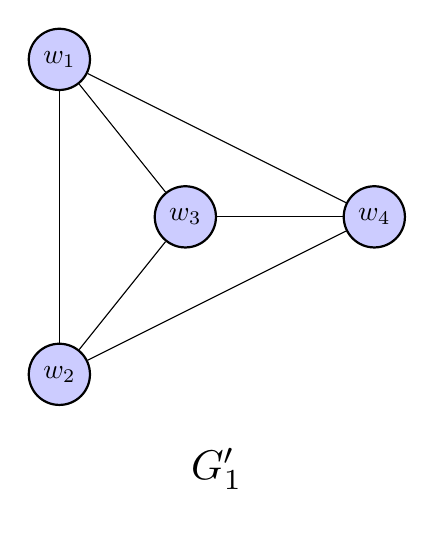
\begin{tikzpicture}[scale=.8,auto=left,every node/.style={circle,fill=blue!20,draw=black,thick}]
  % Vértices G'1
  \node (m1) at (0, 4) {$w_1$};
  \node (m2) at (0, -1) {$w_2$};
  \node (m3) at (2, 1.5) {$w_3$};
  \node (m4) at (5, 1.5) {$w_4$};

  % Aristas G'1
  \foreach \from/\to in {m1/m2, m1/m3, m1/m4, m2/m3, m2/m4, m3/m4}
    \draw (\from) -- (\to);

  % Título
  \node[draw=none, fill=none, scale=1.5] at (2.5, -2.5) {$G'_1$};
\end{tikzpicture}
